%
% 4_Goce.tex
%
% (c) 2020 Prof Dr Andreas Müller, Hochschule Rapperswil
%
% !TEX root = ../../buch.tex
% !TEX encoding = UTF-8
%
\section{GOCE
\label{planet:section:goce}}
\rhead{GOCE}

Die folgenden Angaben zur GOCE-Mission in diesem Abschnitt stammen von \cite{planet:goce}.

\begin{figure}[h]
    \centering
    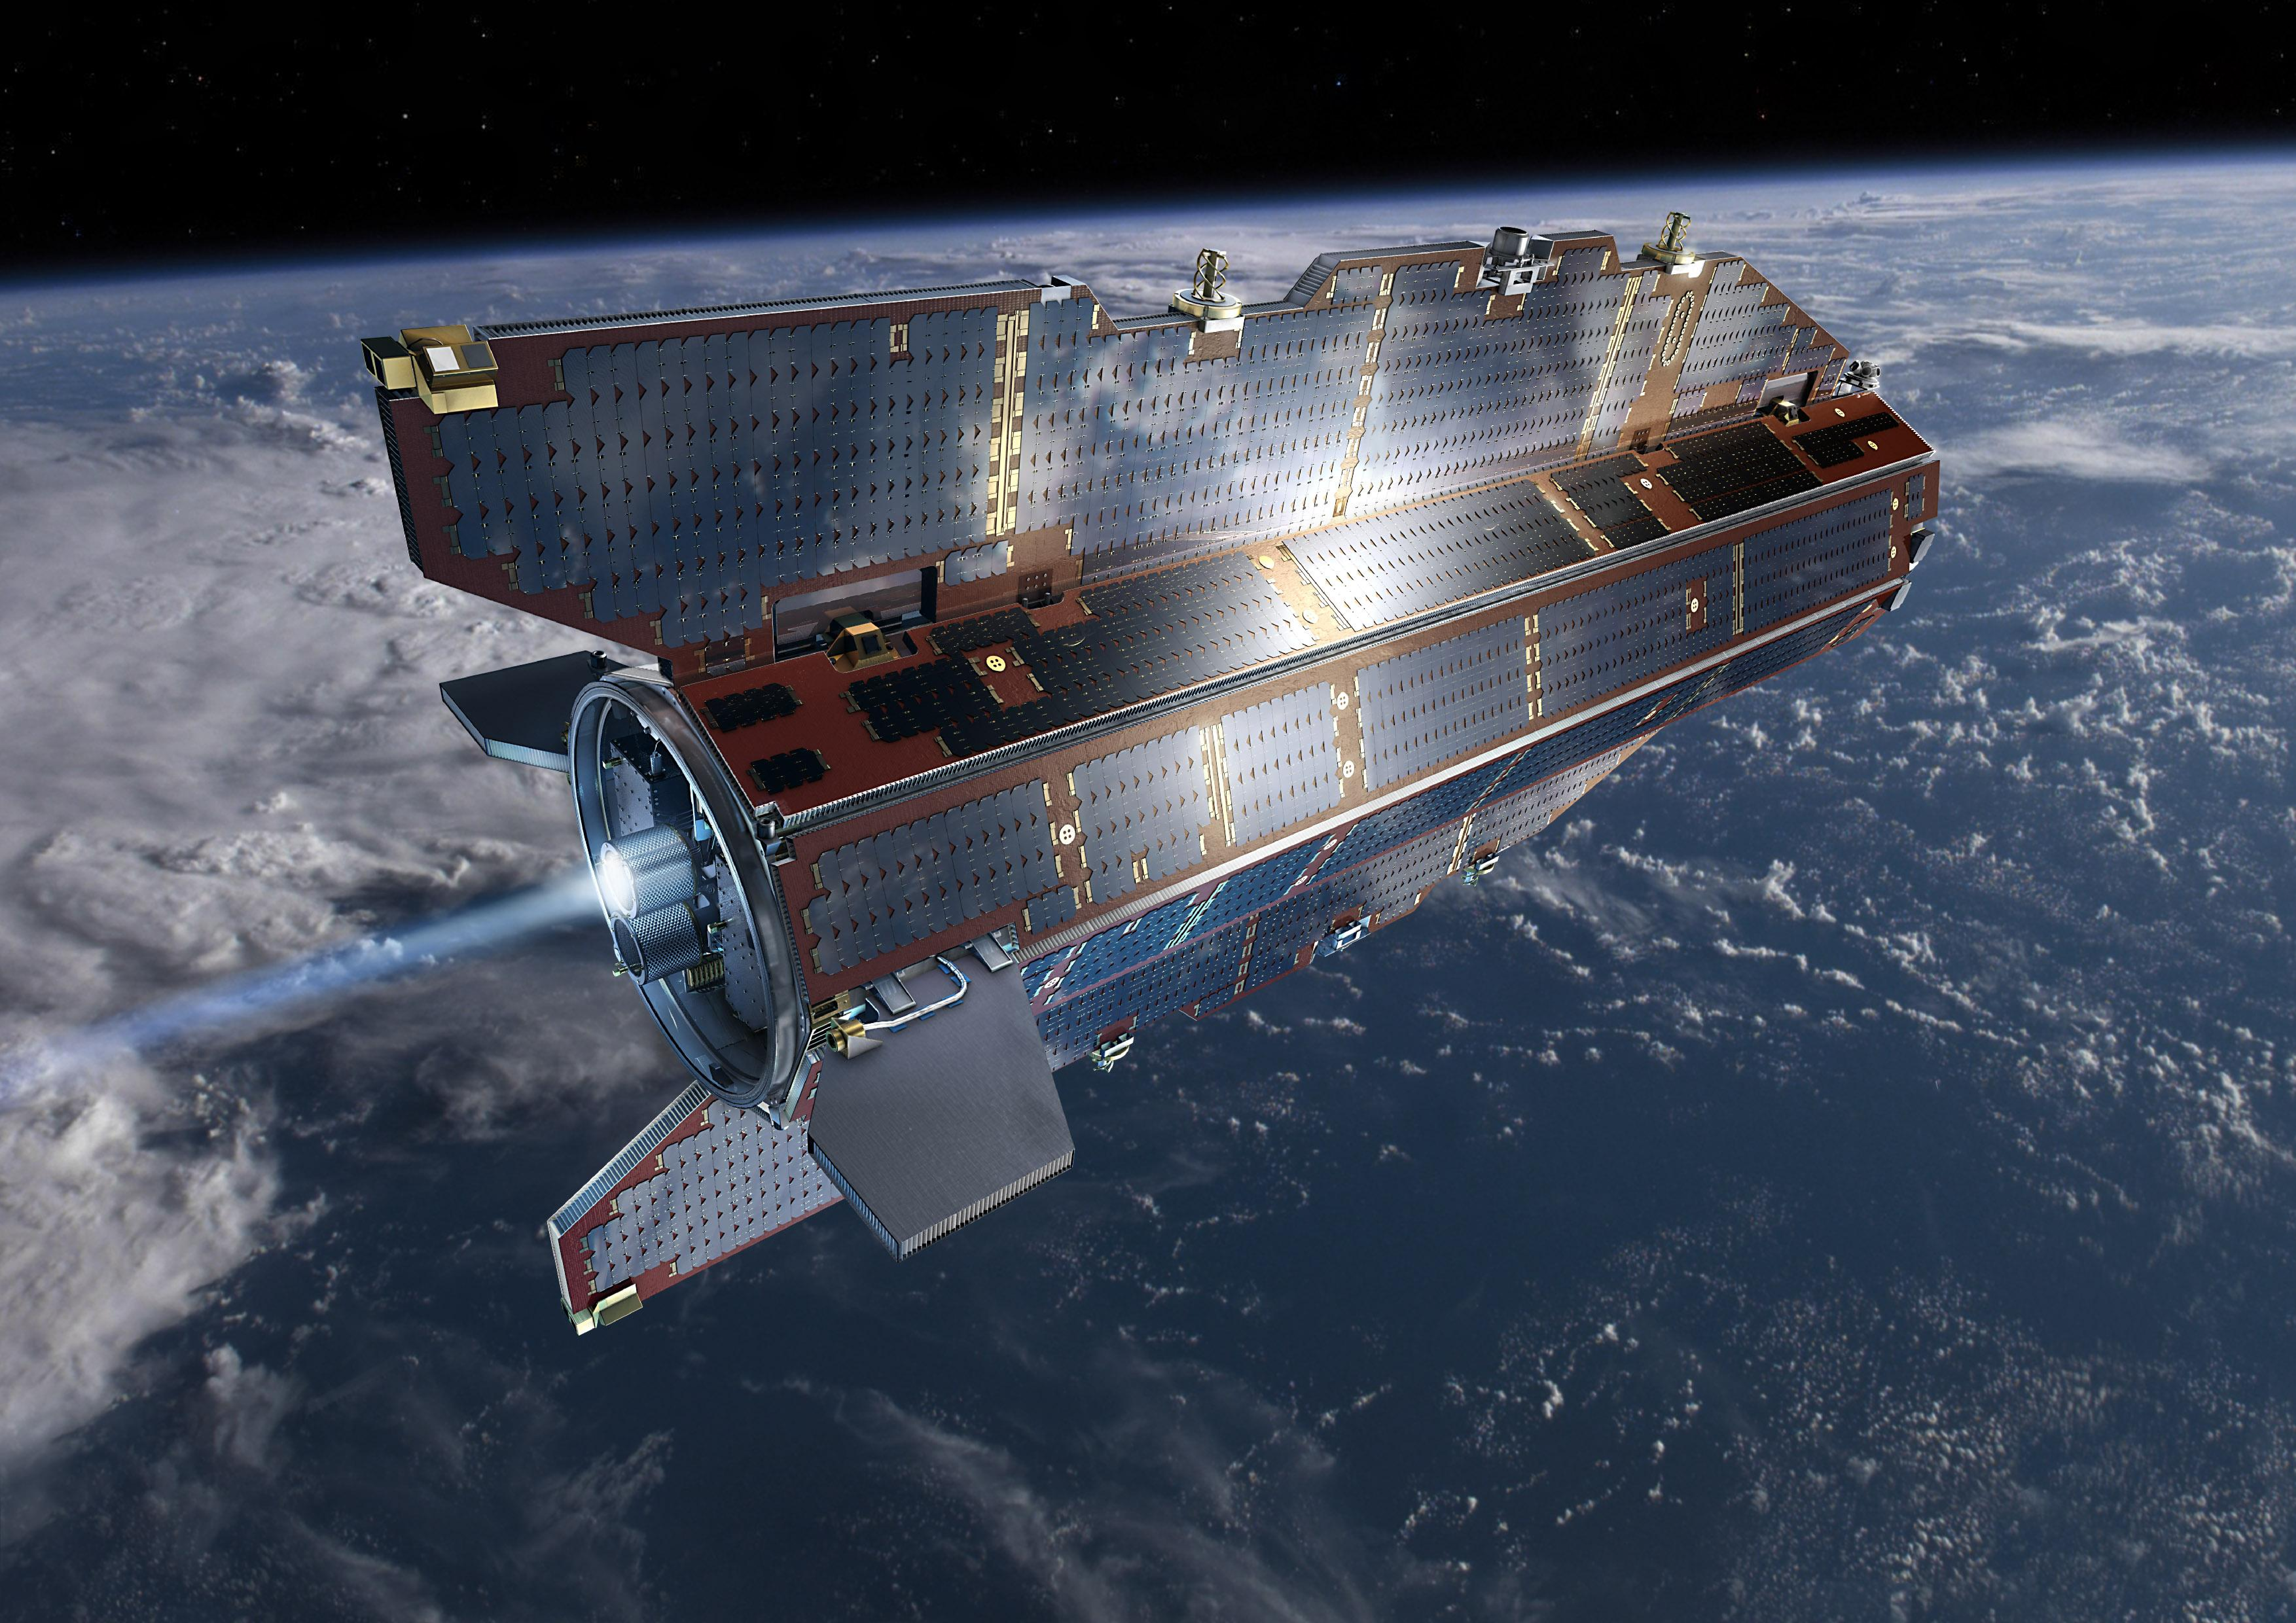
\includegraphics[width=\linewidth]{papers/planet/pictures/goce.pdf}
    \caption{Sattelit aus der GOCE Mission \cite{planet:gocepic}
        \label{planet:fig:goce}}
\end{figure}

Der Gravity Field and Steady-State Ocean Circulation Explorer (GOCE) ist ein Satellit, der im März 2009 von der Europäischen Weltraumorganisation ESA ins Weltall geschickt wurde.
GOCE umkreist die Erde in einer erdnahen Umlaufbahn von nur 260\,km höhe, um das Schwerefeld der Erde mit bisher unerreichter Genauigkeit und räumlicher Auflösung zu erfassen.
Dafür nutzt GOCE einen Gradiometer unterstützt durch GPS um zusätzlich in Echtzeit die Navigation der Umlaufbahn aufzuzeichnen.

Das Gradiometer basiert auf drei Paare von Beschleunigungssensoren.
Das Gradiometer misst den gradienten der Gravitation um eine sehr genaue Erfassung des Geoid der Erde, in \cref{planet:fig:geoid} zusehen.
Dies gibt einen Einblick in die inneren Strukturen der Erde, sowie in die Strömungen in den Tiefen der Ozeane.
Die zweite Funktion des Gradiometer besteht darin die Beschleunigung in Flugrichtung zu messen, damit das Raumschiff nahezu im freiem Fall befindet.

In der \cref{planet:fig:geoid} ist in den gelben Bereichen das Gravitationsfeld höher und in den blauen niedriger.
Aus dem \cref{planet:section:multipol} wird ersichtlich, was die Multipolentwicklung der Kugelform bedeutet, sie beschreiben die Abweichung von der perfekten Kugelform.
Die GOCE-Resultate werden daher mit den Multipolkoeffizienten geliefert.

\begin{figure}[h]
    \centering
    \includegraphics[width=\linewidth]{papers/planet/pictures/geoid.pdf}
    \caption{Darstellung des Gravitationsfeld der Erde \cite{planet:geoidpic}
        \label{planet:fig:geoid}}
\end{figure}


